\section{Ammassi Stellari}
All'interno del cosmo le stelle tendono ad aggregarsi in \emph{ammassi aperti} ed \emph{ammassi globulari}:

\begin{description}
\item[ammassi aperti:]costituite da un numero di stelle che si aggira tra i $10^2$ ed i $10^5$ elementi, tenuti insieme dalla mutua attrazione gravitazionale. Generalmente formate da stelle giovani e orbitano nel disco di galassie a spirale.
\item[ammassi globulari:]invece sono strutture decisamente più grandi, costituite infatti da un numero di stelle che si aggira intorno ai $10^5 - 10^6$. Questi sembrano trovarsi principalmente in orbita attorno agli aloni galattici, ma qualche volta anche attorno ai bulge (sec.~\ref{sec:classificazione-di-hubble}). 
\end{description}

Entrambe queste strutture sono caratterizzate dal fatto di essere costituite da stelle con la stessa età e composizione chimica, benché con masse differenti. Gli ammassi sono infatti degli ottimi luoghi per testare il modello di evoluzione stellare. Il modello che è stato studiato infatti, nel quale si è rappresentato l'andamento dell'evoluzione stellare all'interno dei diagrammi H-R, assume che il confronto tra stelle era possibile se fatto tra corpi di composizione chimica simile.

\begin{center}
    \begin{tikzpicture} [
            blu/.style={rectangle, draw=blue!60, fill=blue!5, very thick, minimum size=5mm},
            red/.style={rectangle, draw=red!60, fill=red!5, very thick, minimum size=5mm},
            green/.style={rectangle, draw=green!60, fill=green!5, very thick, minimum size=5mm},]
        \node[red](1){\footnotesize{Massa, X, Y , Z}};
        \node[blu](2)[right=of 1]{\footnotesize{Modello Stellare}};
        \node[green](3)[right=of 2]{\footnotesize{Evoluzione nel diagramma H-R}};

        \draw[->] (1.east) -- (2.west);
        \draw[->] (2.east) -- (3.west);
    \end{tikzpicture}
\end{center}

\subsection{Isocrone nel piano H-R}\label{sec:isocrone}

Andando a studiare le \emph{isocrone} del piano H-R si analizza il comportamento di stelle di massa differente, alla stessa età. Un esempio è la ZAMS o la figura~\ref{fig:isocrona}.

\begin{figure}
    \centering
    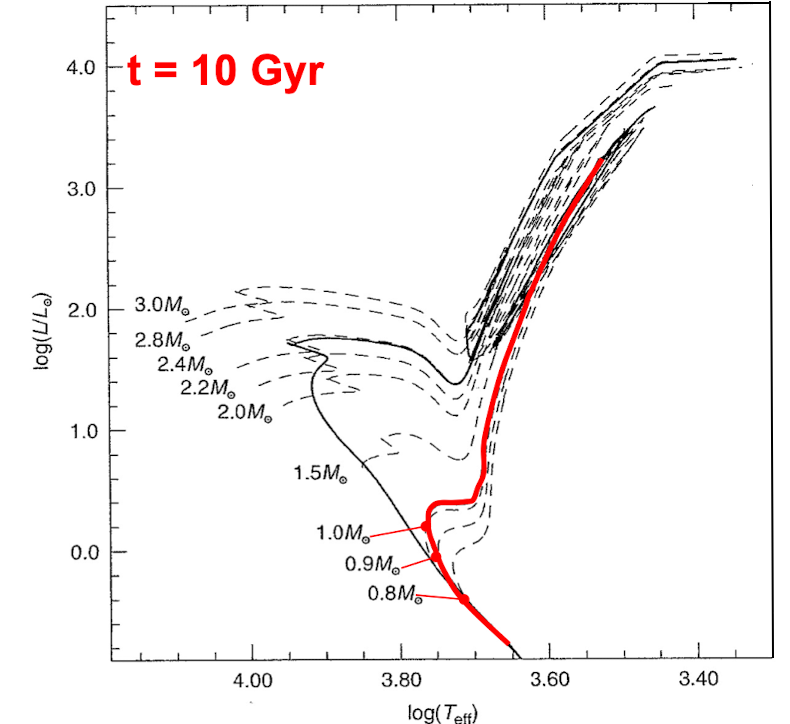
\includegraphics[width = 0.4\textwidth]{immagini/HR-isocrona.png}
    \caption{L'immagine mostra un'isocrona nel piano H-R, in rosso.}\label{fig:isocrona}
\end{figure}
\begin{figure}
    \centering
    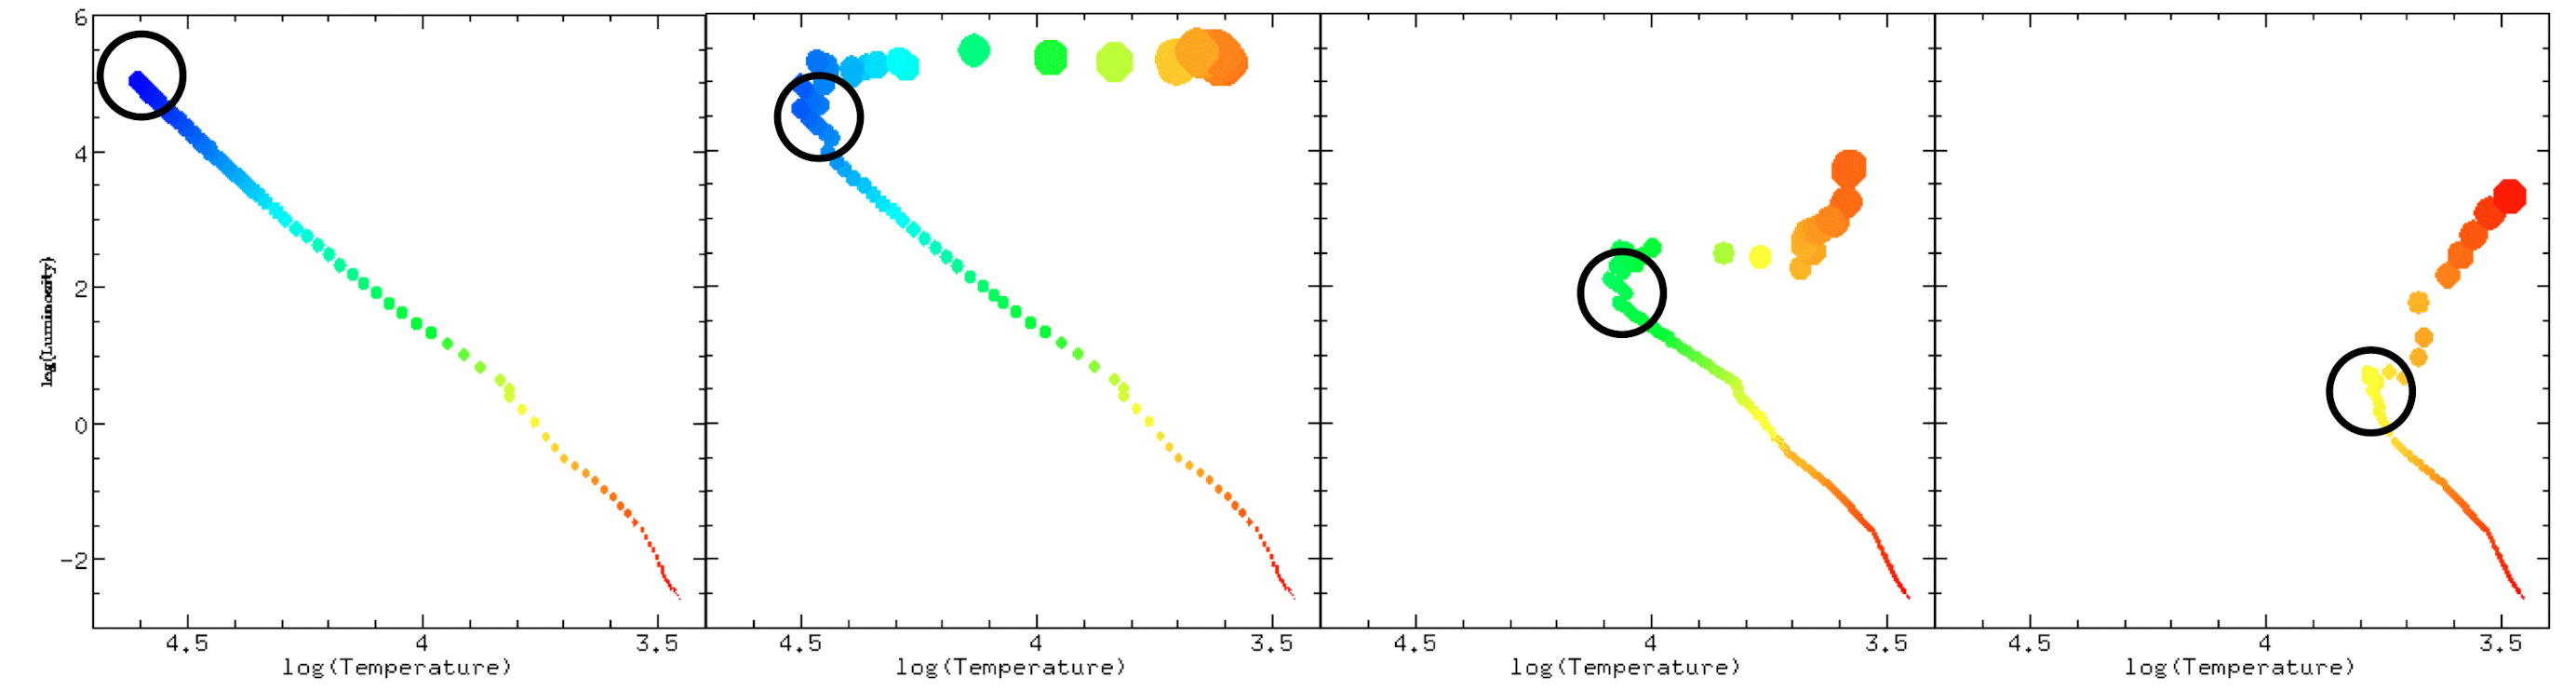
\includegraphics[width = 0.8\textwidth]{immagini/evoluzione-isocrona.png}
    \caption{L'immagine mostra come si evolve l'isocrona del diagramma H-R.}\label{fig:evoluzione-isocrona}
\end{figure}

Si noti, inoltre, come in figura~\ref{fig:evoluzione-isocrona} queste curve diminuiscano di lunghezza. Il motivo risiede nel fatto che all'avanzare del tempo le stelle più pesanti muoiono, infatti la durata della vita è inversamente proporzionale alla massa iniziale.

Si possono ora andare a studiare le sezioni principali di una isocrona. Per composizione chimica fissata ed età crescenti, si raggiungono in sequenza i seguenti punti:

\begin{enumerate}
    \item MS-TO (main sequence turning off point): al diminuire della massa, questo avviene a temperature e luminosità minori;
    \item Forma dell'MS-TO: per stelle con una vita inferiore a $\SI{1}{Gyr}$ la forma è simile a quella di un uncino, mentre stelle con vita superiore da $\SI{1}{Gyr}$ assume una forma più arrotondata;
    \item Estensione della SGB: l'estensione della SGB diminuisce al diminuire della massa iniziale della stella;
    \item Estensione della RGB: al diminuire della massa aumenta il tempo che la stella impiega nel RGB;
    \item luminosità: per stelle con una vita superiore a $\SI{1}{Gyr}$ viene raggiunta una densità costante.
\end{enumerate}
Si può avere un'idea della forma delle varie curve nella figura~\ref{fig:evoluzione-isocrona}, dove però non sono presenti le specificazioni dei vari punti.
\subsection{Prove Sperimentali}

Questo modello teorico rappresenta, però, quello che accade realmente in natura? Per rispondere a questa domanda bisogna però notare che luminosità e temperature non sono grandezze misurabili direttamente. Bisogna quindi costruire un diagramma equivalente a quello H-R per le osservazioni.

La grandezza che è possibile misurare da è la magnitudine apparente di un ammasso di stelle in due o più bande fotometriche (e.g. V e B), ottenendo quindi grandezze come magnitudine e colore. Costruiamo quindi un piano colore-magnitudine (CMD), sul quale posizionare ogni stella di un ammasso. Si ha infatti che il colore è una grandezza fortemente legata alla temperatura, mentre la magnitudine lo è con la luminosità.

Comparando l'andamento teorico e quello sperimentale nei due diagrammi (H-R e CMD) si osserva che effettivamente è presente un'ottima correlazione tra le due forme. Mostrando che effettivamente la risposta alla domanda iniziale è proprio sì, il modello teorico costruito predice in maniera eccellente quello che accade in natura (come mostrato in figura~\ref{fig:modello-osservazione-stellare}).
\begin{figure}
    \centering
    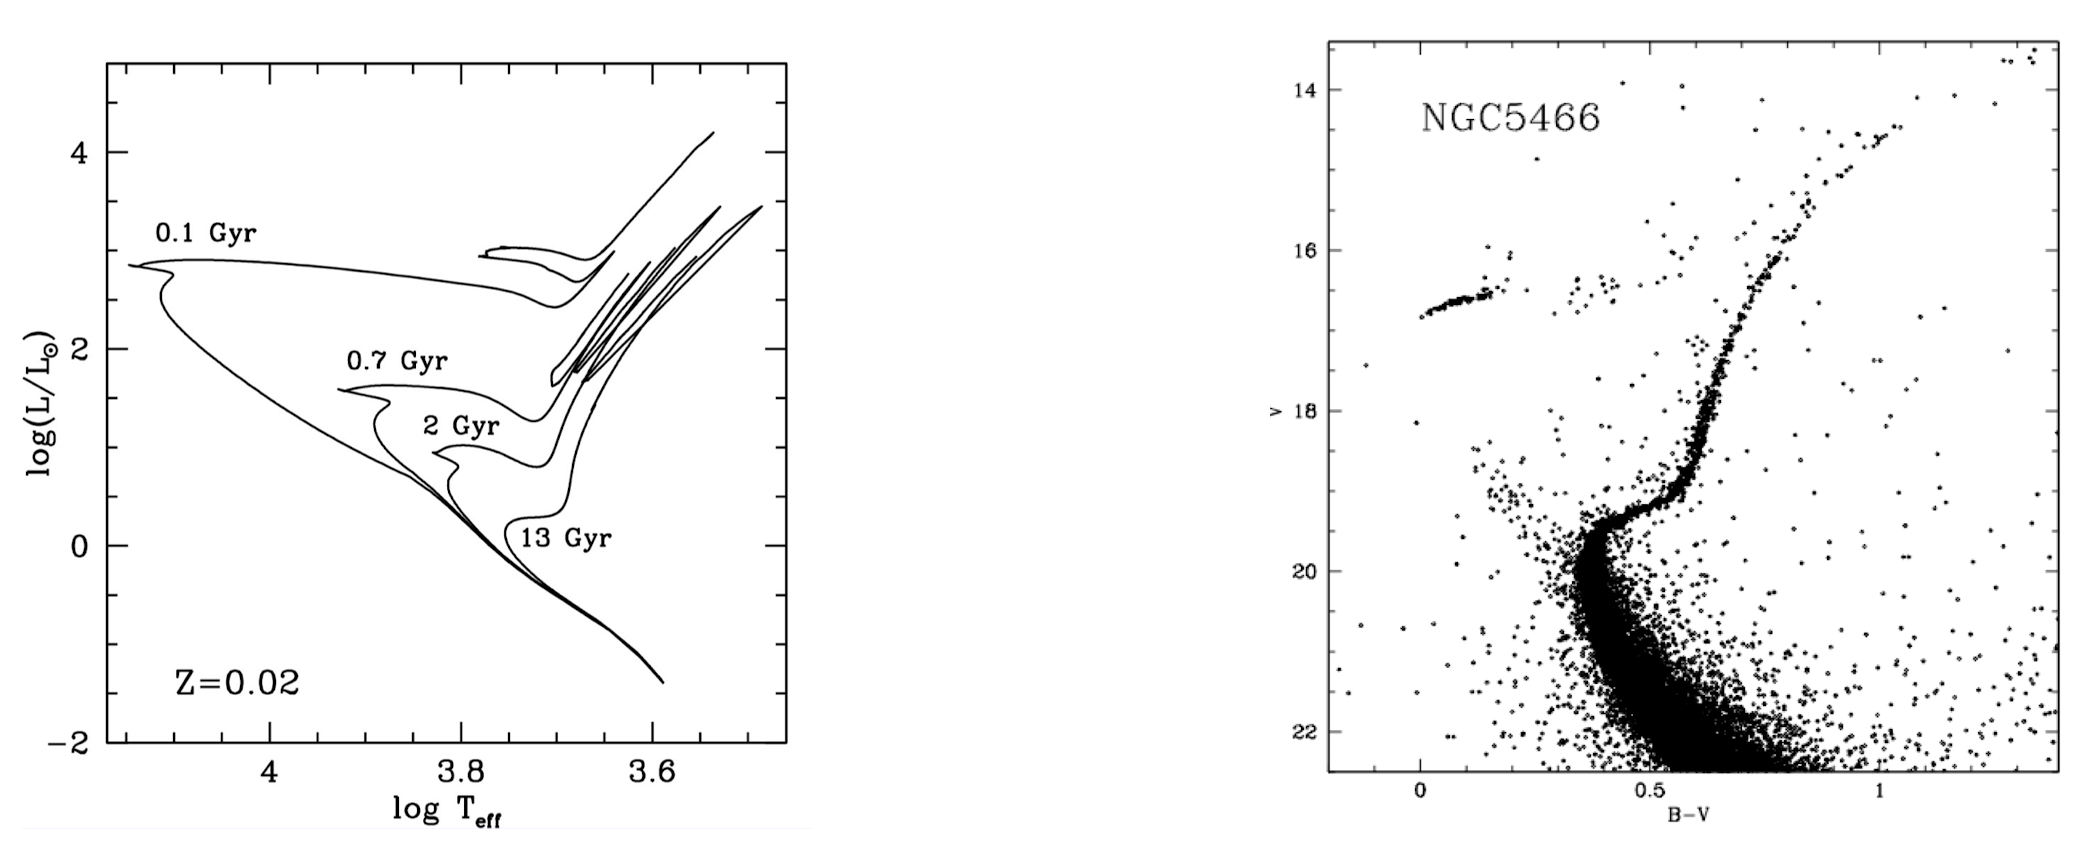
\includegraphics[width = 0.8\textwidth]{immagini/dati-sper-stelle.png}
    \caption{La figura mostra a sinistra l'andamento teorico del modello in un piano H-R, mentre a destra l'andamento dei dati sperimentali relativi a un ammasso stellare, in un piano CMD.}\label{fig:modello-osservazione-stellare}
\end{figure}

Lo studio degli ammassi stellari risulta, quindi, fondamentale per confermare ciò che viene dedotto nello sviluppo dei modelli stellari, ma non solo. Infatti vengono usati anche per l'analisi di alcune caratteristiche fisiche delle galassie, che non sono altro che un insieme di ammassi, ognuno con la propria età e con la propria composizione chimica.

In particolare per galassie abbastanza vicine è possibile utilizzare il CMD, in questo caso si dice che la galassia è \emph{risoluta}, mentre nel caso opposto \emph{non risoluta}. In quest'ultima non si può adoperare lo studio delle stelle per ottenere le proprietà della galassia.